\documentclass{beamer}
\usetheme{Madrid}
\usecolortheme{default}

% Define OSU orange color
\definecolor{osaorange}{RGB}{220,115,38}

% Set colors
\setbeamercolor{structure}{fg=osaorange}
\setbeamercolor{title}{fg=white,bg=osaorange}
\setbeamercolor{frametitle}{fg=white,bg=osaorange}

\usepackage{graphicx}
\usepackage{amsmath}
\usepackage{booktabs}
\usepackage{hyperref}
\usepackage{tikz}
\usetikzlibrary{shapes,arrows}

\title{H524 Introduction to Biostatistics}
\subtitle{Week 6: Power, Two-Sample Tests, and ANOVA}
\author{Dr. John Molitor}
\institute{}
\date{Fall 2025}

\begin{document}

\frame{\titlepage}

\begin{frame}
\frametitle{Outline}
\tableofcontents
\end{frame}

\section{Review from Week 5}

\begin{frame}
\frametitle{Quick Review: Hypothesis Testing}
\textbf{Last week we covered:}
\begin{itemize}
\item Null and alternative hypotheses
\item Test statistics and p-values
\item One-sample t-tests for means
\item Type I error (false positive) and significance level $\alpha$
\item Rejection regions and critical values
\end{itemize}

\vspace{0.5cm}
\textbf{This Week:} Extending hypothesis testing
\begin{itemize}
\item Statistical power and Type II errors
\item Comparing two independent samples
\item Paired samples and dependent data
\item Analysis of Variance (ANOVA) for multiple groups
\end{itemize}

\vspace{0.3cm}
\textbf{Reading:} Pagano \& Gauvreau Chapters 11-12
\end{frame}

\section{Statistical Power (Chapter 11)}

\begin{frame}
\frametitle{Hypothesis Testing Errors}
\textbf{Two types of errors in hypothesis testing:}

\vspace{0.3cm}
\begin{center}
\begin{tabular}{l|cc}
\toprule
 & \multicolumn{2}{c}{\textbf{Truth}} \\
\textbf{Decision} & $H_0$ True & $H_0$ False \\
\midrule
Reject $H_0$ & Type I Error & Correct Decision \\
 & (False Positive) & (True Positive) \\
 & Probability = $\alpha$ & Probability = $1-\beta$ (Power) \\
\midrule
Fail to Reject $H_0$ & Correct Decision & Type II Error \\
 & (True Negative) & (False Negative) \\
 & Probability = $1-\alpha$ & Probability = $\beta$ \\
\bottomrule
\end{tabular}
\end{center}

\vspace{0.5cm}
\textbf{Key Definitions:}
\begin{itemize}
\item $\alpha$ = Type I error rate (significance level, usually 0.05)
\item $\beta$ = Type II error rate (probability of missing real effect)
\item \textbf{Power} = $1 - \beta$ (probability of detecting real effect)
\end{itemize}
\end{frame}

\begin{frame}
\frametitle{What is Statistical Power?}
\textbf{Definition:} Power is the probability of correctly rejecting $H_0$ when it is false.

$$\text{Power} = 1 - \beta = \Pr(\text{Reject } H_0 \mid H_0 \text{ is false})$$

\vspace{0.5cm}
\textbf{Interpretation:}
\begin{itemize}
\item Power = 0.80 means 80\% chance of detecting a real effect
\item If power is too low, you might miss important findings
\item Typically want power $\geq$ 0.80 (80\%)
\item Some fields require power $\geq$ 0.90 (90\%)
\end{itemize}

\vspace{0.5cm}
\textbf{Example:}
\begin{itemize}
\item Testing a new drug vs. placebo
\item Drug truly reduces blood pressure by 10 mmHg
\item Power = 0.80 means 80\% chance our study will detect this effect
\item 20\% chance we'll conclude ``no effect'' (Type II error)
\end{itemize}
\end{frame}

\begin{frame}
\frametitle{Factors Affecting Power}
\textbf{Power increases with:}

\vspace{0.3cm}
\textbf{1. Larger Sample Size ($n$)}
\begin{itemize}
\item More data $\Rightarrow$ smaller standard error $\Rightarrow$ easier to detect effects
\item Most important and controllable factor
\end{itemize}

\vspace{0.3cm}
\textbf{2. Larger Effect Size ($|\mu - \mu_0|$ or $|\mu_1 - \mu_2|$)}
\begin{itemize}
\item Bigger differences are easier to detect
\item Not under researcher's control
\end{itemize}

\vspace{0.3cm}
\textbf{3. Lower Variability ($\sigma$)}
\begin{itemize}
\item Less noise $\Rightarrow$ clearer signal
\item Can be reduced by careful measurement and study design
\end{itemize}

\vspace{0.3cm}
\textbf{4. Higher Significance Level ($\alpha$)}
\begin{itemize}
\item Trade-off: higher $\alpha$ increases power but increases Type I error
\item Usually keep $\alpha = 0.05$ fixed
\end{itemize}
\end{frame}

\begin{frame}
\frametitle{Power Calculation Example}
\textbf{Scenario:} Testing if a new drug lowers cholesterol

\vspace{0.3cm}
\textbf{Given:}
\begin{itemize}
\item Population mean cholesterol: $\mu_0 = 200$ mg/dL
\item We want to detect a reduction to $\mu = 190$ mg/dL
\item Known SD: $\sigma = 30$ mg/dL
\item Sample size: $n = 25$
\item Significance level: $\alpha = 0.05$ (two-sided)
\end{itemize}

\vspace{0.3cm}
\textbf{Question:} What is the power to detect this 10 mg/dL reduction?

\vspace{0.3cm}
\textbf{Solution:}
\begin{enumerate}
\item Standard error: $\text{SE} = 30/\sqrt{25} = 6$ mg/dL
\item Critical value: $z_{0.975} = 1.96$
\item Rejection region: Reject if $\bar{x} < 200 - 1.96(6) = 188.24$ or $\bar{x} > 211.76$
\item Under true $\mu = 190$: Calculate $\Pr(\bar{X} < 188.24 \text{ or } \bar{X} > 211.76 \mid \mu = 190)$
\end{enumerate}
\end{frame}

\begin{frame}[fragile]
\frametitle{Power Calculation in R}
\textbf{Calculate power for the cholesterol example:}

\vspace{0.2cm}
\footnotesize
\begin{verbatim}
# Parameters
mu0 <- 200; mu1 <- 190; sigma <- 30; n <- 25; alpha <- 0.05

# Standard error
se <- sigma / sqrt(n)  # 6

# Critical values (two-sided)
z_crit <- qnorm(1 - alpha/2)  # 1.96
lower_crit <- mu0 - z_crit * se  # 188.24
upper_crit <- mu0 + z_crit * se  # 211.76

# Power: P(reject H0 | mu = 190)
power_lower <- pnorm(lower_crit, mean=mu1, sd=se)
power_upper <- pnorm(upper_crit, mean=mu1, sd=se,
                     lower.tail=FALSE)
power <- power_lower + power_upper
cat("Power:", round(power, 3))  # 0.385
\end{verbatim}
\end{frame}

\begin{frame}
\frametitle{Power Calculation Results}
\textbf{Result:} Power = 0.385 (38.5\%)

\vspace{0.3cm}
\textbf{Interpretation:}
\begin{itemize}
\item Only 38.5\% chance of detecting a 10 mg/dL reduction with $n=25$
\item 61.5\% chance of Type II error (missing the effect)
\item This is too low! We want power $\geq$ 0.80
\end{itemize}

\vspace{0.3cm}
\textbf{Solution:} Increase sample size

\vspace{0.2cm}
For power = 0.80, we need approximately $n = 73$ subjects

\vspace{0.2cm}
\textbf{General lesson:}
\begin{itemize}
\item Always calculate power \textbf{before} conducting study
\item Helps determine necessary sample size
\item Avoids wasting resources on underpowered studies
\item Part of good study design and grant proposals
\end{itemize}
\end{frame}

\begin{frame}[fragile]
\frametitle{Sample Size Calculation in R}
\textbf{Using \texttt{power.t.test()} function:}

\vspace{0.2cm}
\footnotesize
\begin{verbatim}
# Calculate required sample size for power = 0.80
power.t.test(delta = 10,      # Effect size (|mu1 - mu0|)
             sd = 30,          # Standard deviation
             sig.level = 0.05, # Significance level
             power = 0.80,     # Desired power
             type = "one.sample")

# Output:
#      One-sample t test power calculation
#               n = 72.58
#           delta = 10
#              sd = 30
#       sig.level = 0.05
#           power = 0.8
# Need n = 73 subjects
\end{verbatim}
\end{frame}

\begin{frame}[fragile]
\frametitle{Sample Size Calculation in R (continued)}
\textbf{Calculate power for given sample size:}

\vspace{0.2cm}
\footnotesize
\begin{verbatim}
# Can also calculate power for given n
power.t.test(n = 25, delta = 10, sd = 30,
             sig.level = 0.05, type = "one.sample")

# Output:
#      One-sample t test power calculation
#               n = 25
#           delta = 10
#              sd = 30
#       sig.level = 0.05
#           power = 0.360
# Power = 0.360 (slightly lower than z-based calculation)
\end{verbatim}
\end{frame}

\begin{frame}
\frametitle{Power Curves}
\textbf{Visualizing how power changes with sample size:}

\vspace{0.3cm}
\begin{center}
\textit{[Power increases non-linearly with sample size]}
\end{center}

\vspace{0.3cm}
\textbf{Key observations:}
\begin{itemize}
\item Power increases rapidly initially
\item Diminishing returns for very large $n$
\item To double power from 0.40 to 0.80, need $\sim$4x sample size
\item To cut standard error in half, need 4x sample size
\end{itemize}

\vspace{0.5cm}
\textbf{Practical implications:}
\begin{itemize}
\item Small studies ($n < 30$) often severely underpowered
\item ``Pilot studies'' rarely have power to detect effects
\item Need careful planning and power analysis before data collection
\item Consider effect size: smaller effects need larger samples
\end{itemize}
\end{frame}

\section{Two-Sample t-Tests: Independent Samples (Chapter 12)}

\begin{frame}
\frametitle{Comparing Two Independent Groups}
\textbf{Common research questions:}
\begin{itemize}
\item Does treatment A work better than treatment B?
\item Do men and women differ in average blood pressure?
\item Is mean cholesterol higher in smokers vs. non-smokers?
\end{itemize}

\vspace{0.5cm}
\textbf{Two-sample problem:}
\begin{itemize}
\item Two independent groups (treatment/control, male/female, etc.)
\item Want to compare population means: $\mu_1$ vs. $\mu_2$
\item Observe sample means: $\bar{x}_1$ and $\bar{x}_2$
\end{itemize}

\vspace{0.5cm}
\textbf{Hypotheses:}
\begin{align*}
H_0&: \mu_1 = \mu_2 \quad \text{(or equivalently: } \mu_1 - \mu_2 = 0\text{)}\\
H_A&: \mu_1 \neq \mu_2 \quad \text{(two-sided)}
\end{align*}

Or one-sided: $H_A: \mu_1 > \mu_2$ or $H_A: \mu_1 < \mu_2$
\end{frame}

\begin{frame}
\frametitle{Two-Sample t-Test: Assumptions}
\textbf{Assumptions for validity:}

\vspace{0.3cm}
\textbf{1. Independence}
\begin{itemize}
\item Observations within each group are independent
\item The two groups are independent of each other
\item Violated by paired data (covered later)
\end{itemize}

\vspace{0.3cm}
\textbf{2. Normality}
\begin{itemize}
\item Data in each group approximately normal
\item Or large sample sizes ($n_1, n_2 \geq 30$) for CLT
\item Check with histograms, Q-Q plots
\end{itemize}

\vspace{0.3cm}
\textbf{3. Equal Variances (for pooled t-test)}
\begin{itemize}
\item $\sigma_1^2 = \sigma_2^2$ (homogeneity of variance)
\item Can test with F-test or Levene's test
\item If violated, use Welch's t-test (does not assume equal variances)
\end{itemize}
\end{frame}

\begin{frame}
\frametitle{Pooled Two-Sample t-Test}
\textbf{When variances are equal:} $\sigma_1^2 = \sigma_2^2 = \sigma^2$

\vspace{0.3cm}
\textbf{Test statistic:}
$$t = \frac{(\bar{x}_1 - \bar{x}_2) - 0}{s_p \sqrt{\frac{1}{n_1} + \frac{1}{n_2}}}$$

where the \textbf{pooled standard deviation} is:
$$s_p = \sqrt{\frac{(n_1-1)s_1^2 + (n_2-1)s_2^2}{n_1 + n_2 - 2}}$$

\vspace{0.3cm}
\textbf{Distribution:} Under $H_0$, $t \sim t_{n_1 + n_2 - 2}$

\vspace{0.3cm}
\textbf{Degrees of freedom:} $df = n_1 + n_2 - 2$

\vspace{0.3cm}
\textbf{Decision rule:}
\begin{itemize}
\item Calculate p-value: $p = 2 \times \Pr(T > |t| \mid H_0)$ for two-sided
\item Reject $H_0$ if $p < \alpha$
\end{itemize}
\end{frame}

\begin{frame}
\frametitle{Example: Tumor Growth Study}
\textbf{Study:} Effect of new drug on tumor growth (mm/month)

\begin{center}
\renewcommand{\arraystretch}{0.9}
\begin{tabular}{cc}
\toprule
Control & Treatment \\
\midrule
7 & 4 \\
10 & 6 \\
9 & 10 \\
8 & 8 \\
7 & 5 \\
6 & 3 \\
8 & 10 \\
9 & 8 \\
12 & 8 \\
13 & 10 \\
\bottomrule
\end{tabular}
\end{center}

\vspace{0.05cm}
\textbf{Question:} Does the treatment reduce tumor growth?

\small
\textbf{Hypotheses:}
\begin{itemize}
\setlength\itemsep{-0.3em}
\item $H_0: \mu_C = \mu_T$ (no difference)
\item $H_A: \mu_C > \mu_T$ (treatment reduces growth)
\end{itemize}
\end{frame}

\begin{frame}[fragile]
\frametitle{Two-Sample t-Test in R (Part 1 - Setup)}
\small
\begin{verbatim}
# Enter data
control <- c(7, 10, 9, 8, 7, 6, 8, 9, 12, 13)
treatment <- c(4, 6, 10, 8, 5, 3, 10, 8, 8, 10)

# Summary statistics
mean(control)    # 8.9 mm
mean(treatment)  # 7.2 mm
sd(control)      # 2.234 mm
sd(treatment)    # 2.573 mm

# Pooled two-sample t-test (equal variances)
t.test(control, treatment,
       var.equal = TRUE,     # Assume equal variances
       alternative = "greater")  # One-sided: control > treatment
\end{verbatim}
\end{frame}

\begin{frame}[fragile]
\frametitle{Two-Sample t-Test in R (Part 2 - Results)}
\small
\begin{verbatim}
# Output from t.test():
# t = 1.578, df = 18, p-value = 0.066
# mean of x = 8.9, mean of y = 7.2
# 95% CI: (-0.182, Inf)

# Conclusion: p = 0.066 > 0.05, fail to reject H0
# Not enough evidence that treatment reduces growth
\end{verbatim}
\end{frame}

\begin{frame}
\frametitle{Welch's t-Test (Unequal Variances)}
\textbf{When variances are unequal:} $\sigma_1^2 \neq \sigma_2^2$

\vspace{0.3cm}
\textbf{Test statistic:}
$$t = \frac{\bar{x}_1 - \bar{x}_2}{\sqrt{\frac{s_1^2}{n_1} + \frac{s_2^2}{n_2}}}$$

\vspace{0.3cm}
\textbf{Degrees of freedom (Welch-Satterthwaite):}
$$df = \frac{\left(\frac{s_1^2}{n_1} + \frac{s_2^2}{n_2}\right)^2}{\frac{(s_1^2/n_1)^2}{n_1-1} + \frac{(s_2^2/n_2)^2}{n_2-1}}$$

\vspace{0.3cm}
\textbf{In R:} Just use \texttt{t.test()} with \texttt{var.equal = FALSE} (default!)

\vspace{0.3cm}
\textbf{When to use:}
\begin{itemize}
\item Always safer to use Welch's test
\item More robust, similar power when variances equal
\item Default in R's \texttt{t.test()} function
\end{itemize}
\end{frame}

\begin{frame}
\frametitle{Confidence Interval for Difference in Means}
\textbf{95\% CI for $\mu_1 - \mu_2$ (pooled):}

$$(\bar{x}_1 - \bar{x}_2) \pm t_{0.975, df} \times s_p \sqrt{\frac{1}{n_1} + \frac{1}{n_2}}$$

where $df = n_1 + n_2 - 2$

\vspace{0.1cm}
\textbf{Tumor example:}
\begin{itemize}
\setlength\itemsep{-0.3em}
\item $\bar{x}_C - \bar{x}_T = 8.9 - 7.2 = 1.7$ mm
\item $s_p = 2.409$ mm
\item $t_{0.975, 18} = 2.101$
\item $\text{SE} = 2.409 \sqrt{\frac{1}{10} + \frac{1}{10}} = 1.078$ mm
\item 95\% CI: $1.7 \pm 2.101 \times 1.078 = 1.7 \pm 2.26$
\item \textbf{95\% CI: (-0.56, 3.96) mm}
\end{itemize}

\vspace{0.05cm}
\small
\textbf{Interpretation:} We are 95\% confident the true difference is between -0.56 and 3.96 mm. Since interval includes 0, no significant difference at $\alpha = 0.05$.
\end{frame}

\section{Paired t-Tests (Chapter 12)}

\begin{frame}
\frametitle{Paired vs. Independent Samples}
\textbf{Paired (dependent) samples:}
\begin{itemize}
\item Same subjects measured twice (before/after)
\item Matched pairs (twins, siblings, matched cases)
\item Left vs. right measurements on same subject
\end{itemize}

\vspace{0.5cm}
\textbf{Examples:}
\begin{itemize}
\item Blood pressure before and after medication
\item Weight before and after diet intervention
\item Pain score before and after treatment
\item Test scores with two different methods on same students
\end{itemize}

\vspace{0.5cm}
\textbf{Why pairing matters:}
\begin{itemize}
\item Removes between-subject variability
\item More powerful than two-sample t-test
\item Controls for confounding variables
\item \textbf{Mistake:} Using two-sample test on paired data loses power
\end{itemize}
\end{frame}

\begin{frame}
\frametitle{Paired t-Test Procedure}
\textbf{Key idea:} Analyze the \textit{differences}

\vspace{0.2cm}
\textbf{For each pair $i$:}
$$d_i = x_{i,\text{before}} - x_{i,\text{after}}$$

or $d_i = x_{i,1} - x_{i,2}$

\vspace{0.2cm}
\textbf{Then:} Perform one-sample t-test on the differences

\vspace{0.2cm}
\textbf{Hypotheses:}
\begin{align*}
H_0&: \mu_d = 0 \quad \text{(no change)}\\
H_A&: \mu_d \neq 0 \quad \text{(two-sided)}
\end{align*}

\vspace{0.2cm}
\textbf{Test statistic:}
$$t = \frac{\bar{d} - 0}{s_d / \sqrt{n}}$$

where $\bar{d}$ = mean difference, $s_d$ = SD of differences, $n$ = number of pairs

\vspace{0.1cm}
\textbf{Distribution:} Under $H_0$, $t \sim t_{n-1}$
\end{frame}

\begin{frame}
\frametitle{Example: Blood Pressure Medication}
\textbf{Study:} 10 patients, blood pressure measured before and after medication

\vspace{0.3cm}
\begin{center}
\small
\begin{tabular}{cccr}
\toprule
Patient & Before & After & Difference ($d_i$) \\
\midrule
1 & 145 & 138 & 7 \\
2 & 150 & 142 & 8 \\
3 & 148 & 145 & 3 \\
4 & 142 & 138 & 4 \\
5 & 140 & 135 & 5 \\
6 & 146 & 140 & 6 \\
7 & 149 & 142 & 7 \\
8 & 143 & 136 & 7 \\
9 & 147 & 141 & 6 \\
10 & 144 & 138 & 6 \\
\midrule
Mean & 145.4 & 139.5 & 5.9 \\
SD & 3.13 & 3.10 & 1.52 \\
\bottomrule
\end{tabular}
\end{center}

\vspace{0.3cm}
\textbf{Question:} Does medication significantly reduce blood pressure?
\end{frame}

\begin{frame}[fragile]
\frametitle{Paired t-Test in R (Part 1 - Setup)}
\small
\begin{verbatim}
# Enter data
before <- c(145, 150, 148, 142, 140, 146, 149, 143, 147, 144)
after <- c(138, 142, 145, 138, 135, 140, 142, 136, 141, 138)

# Calculate differences
differences <- before - after
mean(differences)  # 5.9 mmHg
sd(differences)    # 1.52 mmHg

# Paired t-test (Method 1: on differences)
t.test(differences, mu = 0, alternative = "greater")

# Paired t-test (Method 2: paired argument)
t.test(before, after, paired = TRUE, alternative = "greater")
\end{verbatim}
\end{frame}

\begin{frame}[fragile]
\frametitle{Paired t-Test in R (Part 2 - Results)}
\small
\begin{verbatim}
# Output from paired t-test:
# t = 12.24, df = 9, p-value = 0.00000032
# mean of differences = 5.9
# 95% CI: (5.05, Inf)

# Conclusion: p < 0.001, strong evidence that
# medication reduces blood pressure by 5.9 mmHg on average
\end{verbatim}
\end{frame}

\begin{frame}
\frametitle{Paired vs. Independent t-Test Comparison}
\textbf{What if we (incorrectly) used two-sample test?}

\vspace{0.3cm}
Using two-sample t-test: $p = 0.115$ (not significant!)

Using paired t-test: $p = 0.0001$ (highly significant!)

\vspace{0.5cm}
\textbf{Why such a big difference?}
\begin{itemize}
\item Pairing removes between-subject variability
\item Standard error is much smaller: $\text{SE} = 2.78/\sqrt{10} = 0.88$
\item Two-sample SE: $\sqrt{8.23^2/10 + 6.86^2/10} = 3.25$ (nearly 4x larger!)
\item Pairing gives much more power
\end{itemize}

\vspace{0.5cm}
\textbf{Lesson:}
\begin{itemize}
\item Always use paired test for paired data
\item Pairing is a powerful design strategy
\item Can dramatically reduce sample size needed
\end{itemize}
\end{frame}

\section{Analysis of Variance (ANOVA) (Chapter 12)}

\begin{frame}
\frametitle{Comparing More Than Two Groups}
\textbf{Limitation of t-tests:} Only compare two groups at a time

\vspace{0.3cm}
\textbf{What if we have 3+ groups?}
\begin{itemize}
\item Compare 3 drug doses: low, medium, high
\item Compare 4 treatment methods
\item Compare outcomes across multiple hospitals
\end{itemize}

\vspace{0.5cm}
\textbf{Naive approach:} Multiple t-tests
\begin{itemize}
\item Compare groups 1 vs. 2, 1 vs. 3, 2 vs. 3, etc.
\item For $k$ groups: $\binom{k}{2} = \frac{k(k-1)}{2}$ comparisons
\item For $k=3$: 3 tests; for $k=4$: 6 tests; for $k=5$: 10 tests
\end{itemize}

\vspace{0.5cm}
\textbf{Problem: Multiple testing inflation}
\begin{itemize}
\item Each test has Type I error rate $\alpha = 0.05$
\item Overall Type I error rate much higher!
\item For 3 independent tests: $1 - (1-0.05)^3 = 0.143$ (14.3\%)
\item Need a method that controls overall error rate
\end{itemize}
\end{frame}

\begin{frame}
\frametitle{Analysis of Variance (ANOVA)}
\textbf{Solution:} One omnibus test for all groups

\vspace{0.1cm}
\textbf{Hypotheses:}
\begin{align*}
H_0&: \mu_1 = \mu_2 = \cdots = \mu_k \quad \text{(all means equal)}\\
H_A&: \text{At least one mean differs}
\end{align*}

\vspace{0.1cm}
\textbf{Key idea:} Compare variation \textit{between} groups to variation \textit{within} groups

\vspace{0.1cm}
\begin{itemize}
\setlength\itemsep{-0.3em}
\item \textbf{Between-group:} How different are the group means?
\item \textbf{Within-group:} How variable within each group?
\end{itemize}

\vspace{0.1cm}
\textbf{If $H_0$ is true:}
\begin{itemize}
\setlength\itemsep{-0.3em}
\item All groups sampled from same population
\item Between-group $\approx$ within-group variation
\item Differences just due to chance
\end{itemize}

\textbf{If $H_A$ is true:}
\begin{itemize}
\setlength\itemsep{-0.3em}
\item Between-group $>$ within-group variation
\item Group means genuinely different
\end{itemize}
\end{frame}

\begin{frame}
\frametitle{ANOVA: Partitioning Variability (Part 1)}
\textbf{Total variability} = Between-group + Within-group

\vspace{0.3cm}
\textbf{Sum of Squares decomposition:}

$$\text{SS}_{\text{Total}} = \text{SS}_{\text{Between}} + \text{SS}_{\text{Within}}$$

\vspace{0.3cm}
\textbf{Total Sum of Squares:}
$$\text{SS}_{\text{Total}} = \sum_{i=1}^{k}\sum_{j=1}^{n_i} (x_{ij} - \bar{x})^2$$

where $x_{ij}$ = observation $j$ in group $i$, $\bar{x}$ = overall mean
\end{frame}

\begin{frame}
\frametitle{ANOVA: Partitioning Variability (Part 2)}
\textbf{Between-Group Sum of Squares:}
$$\text{SS}_{\text{Between}} = \sum_{i=1}^{k} n_i (\bar{x}_i - \bar{x})^2$$

where $\bar{x}_i$ = mean of group $i$

\vspace{0.3cm}
\textbf{Within-Group Sum of Squares:}
$$\text{SS}_{\text{Within}} = \sum_{i=1}^{k}\sum_{j=1}^{n_i} (x_{ij} - \bar{x}_i)^2$$

Measures variation of observations around their group means
\end{frame}

\begin{frame}
\frametitle{ANOVA: Mean Squares and F-Statistic}
\textbf{Mean Squares} = Sum of Squares / degrees of freedom

\vspace{0.1cm}
\textbf{Between-Group Mean Square:}
$$\text{MS}_{\text{Between}} = \frac{\text{SS}_{\text{Between}}}{k-1}$$

\textbf{Within-Group Mean Square (pooled variance):}
$$\text{MS}_{\text{Within}} = \frac{\text{SS}_{\text{Within}}}{n-k}$$

\small where $k$ = number of groups, $n$ = total sample size

\vspace{0.1cm}
\textbf{F-Statistic:}
$$F = \frac{\text{MS}_{\text{Between}}}{\text{MS}_{\text{Within}}}$$

\vspace{0.1cm}
\textbf{Distribution:} Under $H_0$, $F \sim F_{k-1, n-k}$

\vspace{0.1cm}
\textbf{Decision rule:}
\begin{itemize}
\setlength\itemsep{-0.2em}
\item Large $F$ $\Rightarrow$ evidence against $H_0$
\item Calculate p-value: $p = \Pr(F_{k-1,n-k} > F_{\text{obs}})$
\item Reject $H_0$ if $p < \alpha$
\end{itemize}
\end{frame}

\begin{frame}
\frametitle{ANOVA Table}
\textbf{Standard ANOVA output format:}

\vspace{0.3cm}
\begin{center}
\begin{tabular}{lcccc}
\toprule
Source & SS & df & MS & F \\
\midrule
Between Groups & $\text{SS}_{\text{Between}}$ & $k-1$ & $\text{MS}_{\text{Between}}$ & $F$ \\
Within Groups & $\text{SS}_{\text{Within}}$ & $n-k$ & $\text{MS}_{\text{Within}}$ & \\
\midrule
Total & $\text{SS}_{\text{Total}}$ & $n-1$ & & \\
\bottomrule
\end{tabular}
\end{center}

\vspace{0.5cm}
\textbf{Interpretation:}
\begin{itemize}
\item Large F-statistic $\Rightarrow$ between-group variation is large relative to within-group
\item Small p-value $\Rightarrow$ reject $H_0$, conclude at least one mean differs
\item If reject $H_0$: Follow up with post-hoc tests to see which groups differ
\end{itemize}

\vspace{0.3cm}
\textbf{Note:} ANOVA tells us there's a difference somewhere, but not where!
\end{frame}

\begin{frame}
\frametitle{ANOVA Assumptions}
\textbf{For valid ANOVA results:}

\vspace{0.1cm}
\textbf{1. Independence}
\begin{itemize}
\setlength\itemsep{-0.2em}
\item Observations within and between groups are independent
\item Random sampling or random assignment
\end{itemize}

\vspace{0.1cm}
\textbf{2. Normality}
\begin{itemize}
\setlength\itemsep{-0.2em}
\item Data within each group approximately normal
\item Robust to violations with large samples (CLT)
\item Check with histograms, Q-Q plots
\end{itemize}

\vspace{0.1cm}
\textbf{3. Equal Variances (Homogeneity)}
\begin{itemize}
\setlength\itemsep{-0.2em}
\item $\sigma_1^2 = \sigma_2^2 = \cdots = \sigma_k^2$
\item Check with Levene's test or Bartlett's test
\item Visually: boxplots should have similar spreads
\item If violated: Use Welch's ANOVA or transformation
\end{itemize}

\vspace{0.1cm}
\textbf{4. Balanced Design (preferred but not required)}
\begin{itemize}
\setlength\itemsep{-0.2em}
\item Equal sample sizes in each group increases power
\end{itemize}
\end{frame}

\begin{frame}
\frametitle{Example: Drug Dose Study}
\textbf{Study:} Effect of 3 drug doses on cholesterol reduction (mg/dL)

\vspace{0.1cm}
\begin{center}
\begin{tabular}{ccc}
\toprule
Low Dose & Medium Dose & High Dose \\
\midrule
10 & 15 & 25 \\
12 & 18 & 28 \\
8 & 16 & 30 \\
11 & 20 & 26 \\
9 & 17 & 27 \\
\midrule
Mean: 10.0 & Mean: 17.2 & Mean: 27.2 \\
SD: 1.58 & SD: 1.92 & SD: 1.92 \\
\bottomrule
\end{tabular}
\end{center}

\vspace{0.1cm}
\textbf{Question:} Is there a significant difference in cholesterol reduction across doses?

\vspace{0.1cm}
\textbf{Hypotheses:}
\begin{itemize}
\setlength\itemsep{-0.2em}
\item $H_0: \mu_{\text{low}} = \mu_{\text{med}} = \mu_{\text{high}}$
\item $H_A:$ At least one mean differs
\end{itemize}
\end{frame}

\begin{frame}[fragile]
\frametitle{ANOVA in R (Part 1 - Setup)}
\footnotesize
\begin{verbatim}
# Enter data
low <- c(10, 12, 8, 11, 9)
medium <- c(15, 18, 16, 20, 17)
high <- c(25, 28, 30, 26, 27)

# Create data frame
cholesterol <- c(low, medium, high)
dose <- factor(rep(c("Low", "Medium", "High"), each=5),
               levels=c("Low", "Medium", "High"))
data <- data.frame(cholesterol, dose)

# Perform ANOVA
model <- aov(cholesterol ~ dose, data=data)
summary(model)
\end{verbatim}
\end{frame}

\begin{frame}[fragile]
\frametitle{ANOVA in R (Part 2 - Results)}
\footnotesize
\begin{verbatim}
# Output from summary(model):
#             Df Sum Sq Mean Sq F value Pr(>F)
# dose         2  746.1   373.1   113.1  1.64e-08 ***
# Residuals   12   39.6     3.3

# Conclusion: F(2,12) = 113.1, p < 0.001
# Strong evidence that at least one dose differs
\end{verbatim}
\end{frame}

\begin{frame}
\frametitle{Post-Hoc Tests}
\textbf{After significant ANOVA:} Which groups differ?

\vspace{0.2cm}
\textbf{Problem:} Multiple pairwise comparisons inflates Type I error

\vspace{0.2cm}
\textbf{Solution:} Post-hoc tests that control family-wise error rate

\vspace{0.2cm}
\textbf{Common post-hoc tests:}

\vspace{0.2cm}
\textbf{1. Tukey's HSD (Honestly Significant Difference)}
\begin{itemize}
\setlength\itemsep{-0.2em}
\item Most common and powerful
\item Controls overall Type I error at $\alpha$
\item All pairwise comparisons
\end{itemize}

\vspace{0.2cm}
\textbf{2. Bonferroni Correction}
\begin{itemize}
\setlength\itemsep{-0.2em}
\item Simple but conservative
\item Use $\alpha^* = \alpha / m$ for each test (m = number of comparisons)
\item For 3 groups: $\alpha^* = 0.05/3 = 0.0167$
\end{itemize}

\vspace{0.2cm}
\textbf{3. Scheffe's Method}
\begin{itemize}
\setlength\itemsep{-0.2em}
\item Most conservative
\item Allows any contrasts, not just pairwise
\end{itemize}
\end{frame}

\begin{frame}[fragile]
\frametitle{Post-Hoc Tests in R (Part 1 - Tukey's HSD)}
\small
\begin{verbatim}
# Tukey's HSD test
TukeyHSD(model)

# Output:
#   Tukey multiple comparisons of means
#     95% family-wise confidence level
#
# Fit: aov(formula = cholesterol ~ dose, data = data)
#
# $dose
#                    diff       lwr      upr     p adj
# Medium-Low      7.2000   4.413   10.0870  0.000032
# High-Low       17.2000  14.413   19.9870  0.000000
# High-Medium    10.0000   7.213   12.7870  0.000001

# All pairwise differences are significant
# High dose reduces cholesterol significantly more than
# medium dose, which reduces more than low dose
\end{verbatim}
\end{frame}

\begin{frame}[fragile]
\frametitle{Post-Hoc Tests in R (Part 2 - Alternative)}
\small
\begin{verbatim}
# Alternative: Pairwise t-tests with Bonferroni correction
pairwise.t.test(data$cholesterol, data$dose,
                p.adjust.method = "bonferroni")

# Output:
#         Low    Medium
# Medium  3.2e-5  -
# High    < 2e-16 9.5e-7

# Results are similar to Tukey's HSD
# All pairwise differences remain highly significant
\end{verbatim}
\end{frame}

\begin{frame}
\frametitle{ANOVA vs. Multiple t-Tests}
\textbf{Why ANOVA instead of multiple t-tests?}

\vspace{0.5cm}
\textbf{Advantages of ANOVA:}
\begin{enumerate}
\item \textbf{Controls Type I error rate}
\begin{itemize}
\item One test at $\alpha = 0.05$ level
\item Multiple t-tests inflate error rate
\end{itemize}

\item \textbf{More powerful}
\begin{itemize}
\item Pools variance estimate across all groups
\item More degrees of freedom for error
\end{itemize}

\item \textbf{Can test complex hypotheses}
\begin{itemize}
\item Test overall effect of categorical variable
\item Can include multiple factors (two-way ANOVA)
\end{itemize}

\item \textbf{Provides comprehensive summary}
\begin{itemize}
\item Single test answers overall question
\item Follow up only if significant
\end{itemize}
\end{enumerate}

\vspace{0.3cm}
\textbf{When to use t-test:} Only 2 groups to compare
\end{frame}

\section{Summary and Key Formulas}

\begin{frame}
\frametitle{Choosing the Right Test}
\textbf{Decision tree:}
\begin{center}
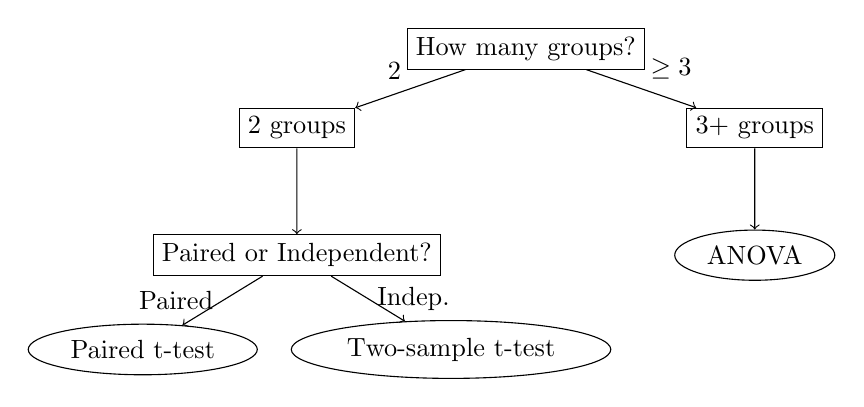
\begin{tikzpicture}[node distance=1.5cm, auto, scale=0.95, every node/.style={transform shape}]
\node (start) [draw, rectangle] {How many groups?};
\node (two) [draw, rectangle, below left of=start, xshift=-2cm] {2 groups};
\node (many) [draw, rectangle, below right of=start, xshift=2cm] {3+ groups};
\node (paired) [draw, rectangle, below of=two, yshift=-0.2cm] {Paired or Independent?};
\node (pairedt) [draw, ellipse, below left of=paired, xshift=-1cm, yshift=-0.2cm] {Paired t-test};
\node (indept) [draw, ellipse, below right of=paired, xshift=1cm, yshift=-0.2cm] {Two-sample t-test};
\node (anova) [draw, ellipse, below of=many, yshift=-0.2cm] {ANOVA};

\draw[->] (start) -- (two) node[midway, above left] {2};
\draw[->] (start) -- (many) node[midway, above right] {$\geq 3$};
\draw[->] (two) -- (paired);
\draw[->] (paired) -- (pairedt) node[midway, left] {Paired};
\draw[->] (paired) -- (indept) node[midway, right] {Indep.};
\draw[->] (many) -- (anova);
\end{tikzpicture}
\end{center}

\footnotesize
\textbf{Additional considerations:}
\begin{itemize}
\setlength\itemsep{-0.4em}
\item Equal variances? Use pooled vs. Welch's t-test
\item Normal data? If not, non-parametric tests (Week 7)
\item Small samples + non-normal? Use caution
\end{itemize}
\end{frame}

\begin{frame}
\frametitle{Key Formulas: Power and Sample Size}
\textbf{Type I and Type II Errors:}
\begin{itemize}
\item $\alpha$ = P(Reject $H_0 \mid H_0$ true) = Type I error
\item $\beta$ = P(Fail to reject $H_0 \mid H_0$ false) = Type II error
\item Power = $1 - \beta$ = P(Reject $H_0 \mid H_0$ false)
\end{itemize}

\vspace{0.3cm}
\textbf{Power depends on:}
\begin{itemize}
\item Sample size $n$ (larger $\Rightarrow$ more power)
\item Effect size $|\mu_1 - \mu_0|$ (larger $\Rightarrow$ more power)
\item Variability $\sigma$ (smaller $\Rightarrow$ more power)
\item Significance level $\alpha$ (larger $\Rightarrow$ more power, but more Type I error)
\end{itemize}

\vspace{0.3cm}
\textbf{In R:}
\begin{itemize}
\item \texttt{power.t.test()} for one-sample and two-sample
\item Specify any 4 of: n, delta, sd, sig.level, power
\item Function solves for the missing parameter
\end{itemize}
\end{frame}

\begin{frame}
\frametitle{Key Formulas: Two-Sample t-Test}
\textbf{Pooled two-sample t-test (equal variances):}

$$t = \frac{\bar{x}_1 - \bar{x}_2}{s_p \sqrt{\frac{1}{n_1} + \frac{1}{n_2}}} \quad \text{where} \quad s_p = \sqrt{\frac{(n_1-1)s_1^2 + (n_2-1)s_2^2}{n_1+n_2-2}}$$

Distribution: $t \sim t_{n_1+n_2-2}$ under $H_0: \mu_1 = \mu_2$

\vspace{0.3cm}
\textbf{Confidence interval for $\mu_1 - \mu_2$:}
$$(\bar{x}_1 - \bar{x}_2) \pm t_{\alpha/2, n_1+n_2-2} \times s_p\sqrt{\frac{1}{n_1} + \frac{1}{n_2}}$$

\vspace{0.3cm}
\textbf{Welch's t-test (unequal variances):}
$$t = \frac{\bar{x}_1 - \bar{x}_2}{\sqrt{\frac{s_1^2}{n_1} + \frac{s_2^2}{n_2}}}$$

with complicated df formula (R calculates automatically)
\end{frame}

\begin{frame}
\frametitle{Key Formulas: Paired t-Test}
\textbf{Paired t-test:}

For differences $d_i = x_{i,1} - x_{i,2}$:

$$t = \frac{\bar{d}}{s_d/\sqrt{n}}$$

where $\bar{d}$ = mean difference, $s_d$ = SD of differences

Distribution: $t \sim t_{n-1}$ under $H_0: \mu_d = 0$

\vspace{0.3cm}
\textbf{Confidence interval for $\mu_d$:}
$$\bar{d} \pm t_{\alpha/2, n-1} \times \frac{s_d}{\sqrt{n}}$$

\vspace{0.3cm}
\textbf{When to use:}
\begin{itemize}
\item Before/after measurements on same subjects
\item Matched pairs (twins, siblings, matched controls)
\item Left/right measurements
\item Any dependent samples
\end{itemize}
\end{frame}

\begin{frame}
\frametitle{Key Formulas: ANOVA}
\textbf{F-statistic:}
$$F = \frac{\text{MS}_{\text{Between}}}{\text{MS}_{\text{Within}}} = \frac{\text{SS}_{\text{Between}}/(k-1)}{\text{SS}_{\text{Within}}/(n-k)}$$

Distribution: $F \sim F_{k-1, n-k}$ under $H_0: \mu_1 = \cdots = \mu_k$

\vspace{0.3cm}
\textbf{Sum of squares:}
\begin{align*}
\text{SS}_{\text{Total}} &= \sum_i\sum_j (x_{ij} - \bar{x})^2\\
\text{SS}_{\text{Between}} &= \sum_i n_i(\bar{x}_i - \bar{x})^2\\
\text{SS}_{\text{Within}} &= \sum_i\sum_j (x_{ij} - \bar{x}_i)^2
\end{align*}

\vspace{0.3cm}
\textbf{Relationship:} $\text{SS}_{\text{Total}} = \text{SS}_{\text{Between}} + \text{SS}_{\text{Within}}$

\vspace{0.3cm}
\textbf{Post-hoc:} If F-test significant, use Tukey's HSD or Bonferroni to identify which groups differ
\end{frame}

\begin{frame}
\frametitle{Summary: This Week}
\textbf{Today we covered:}
\begin{itemize}
\item \textbf{Chapter 11: Power}
  \begin{itemize}
  \item Type I and Type II errors
  \item Statistical power and factors affecting it
  \item Sample size calculations
  \end{itemize}
\item \textbf{Chapter 12: Two-Sample Tests}
  \begin{itemize}
  \item Independent two-sample t-test (pooled and Welch's)
  \item Paired t-test for dependent samples
  \item Confidence intervals for differences
  \end{itemize}
\item \textbf{Chapter 12: ANOVA}
  \begin{itemize}
  \item Comparing 3+ groups simultaneously
  \item F-test and ANOVA table
  \item Post-hoc tests (Tukey, Bonferroni)
  \end{itemize}
\end{itemize}

\vspace{0.5cm}
\textbf{Next Week:} Non-parametric tests (Chapter 13)

\vspace{0.3cm}
\textbf{Reading:} Chapter 13 (Wilcoxon, Kruskal-Wallis, Sign test)
\end{frame}

\begin{frame}
\frametitle{Questions?}
\begin{center}
\Large{Thank you!}

\vspace{1cm}

\textbf{Email:} john.molitor@oregonstate.edu\\
\textbf{Office:} 153 Milam
\end{center}
\end{frame}

\end{document}
